\documentclass[
	12pt,
	a4paper,
	onepage,
	brazil
]{article}

\usepackage[brazil]{babel}
\usepackage[utf8]{inputenc}
\usepackage[T1]{fontenc}
\usepackage{lmodern}
\usepackage{hyperref}
\usepackage{amsmath}
\usepackage{amsthm}
\usepackage{amsfonts}
\usepackage{indentfirst}
\usepackage[most]{tcolorbox}
\usepackage{inconsolata}
\usepackage{caption}
\usepackage{floatrow}
\usepackage[lined,algonl,ruled]{algorithm2e}
\usepackage{float}
\usepackage{graphicx,url}
\usepackage{times,epsfig}
\usepackage[backend=biber, style=numeric]{biblatex}
\addbibresource{tp1.bib}
\usepackage{xcolor}
\hypersetup{
	colorlinks,
	linkcolor={red!50!black},
	urlcolor={red!80!black}
}

\usepackage[
	lmargin = 25mm,
	rmargin = 25mm,
	tmargin = 25mm,
	bmargin = 25mm
]{geometry}

\sloppy

\author{Pedro Otávio Machado Ribeiro}
\title{Trabalho Prático 1\\Entregando Lanches\\Algoritmos e Estruturas de Dados III - 2017/01}
\date{21/05/2017}

\theoremstyle{definition}
\newtheorem{definition}{Definição}

\begin{document}

	\maketitle
	
	\section{Introdução}
	
	Neste trabalho, temos como contexto a empresa de lanches de Rada que realiza as entregas por meio de ciclistas e contratou Gilmar para trabalhar no setor de logística. Num certo momento, a nova prefeita Dora decidiu diminuir a pista de ciclistas para aumentar o tráfego de véiculos automotores, atrapalhando o negócio de lanches de Rada. Dessa forma, dado a posição das franquias de Rada na cidade e dos clientes, as ruas que possuem ciclofaixas e suas respectivas capacidades de tráfego de ciclista e que cada franquia possui uma quantidade arbitráriamente grande de ciclistas, o nosso objetivo é ajudar Gilmar a encontrar a quantidade máxima de ciclistas que podem sair das franquias de realizar as entregas de forma segura. Para que desenvolver a solução, segue abaixo alguns conceitos necessários.
	
	\subsection{Grafo}
	
	Um grafo direcionado ponderado $G$ é uma estrutura matemática definida por um par ordenado $G = (V,E)$, onde $V$ é um conjunto finito de vértices e $E$ uma relação binária em $V$ definida por $(u,v)$ onde $u,v \in V$ que representa uma aresta que sai de $u$ e vai para $v$. Dizemos que $v$ é adjacente à $u$. Além disso, tome $\rho$ a função de custo da aresta definida como segue:
	\begin{align*}
	\rho \colon  V\times V &\to \mathbb{R} \\
	(u,v) &\mapsto c
	\end{align*}
	Neste trabalho, utilizaremos apenas custos $c \in \mathbb{Z}$.
	
	\subsubsection{BFS e DFS}
	
	O BFS(Breadth-first search) é um algoritmo de busca em grafos que prioriza a visita em todos os vértices adjacentes. Dessa forma, sempre que um vértice é visitado, está foi a primeira, e assim temos o menor caminho até ele a partir de uma dada raiz. A visita dos vértices no BFS segue a ordem \textbf{FIFO} e é implementado com uma fila.
	
	O DFS(Deapth-first search) é outro algoritmo de busca. Diferente do BFS, o DFS prioriza a busca
	pelos vértices mais recentes descobertos, de forma que a busca seja a mais profunda possível. Ao chegar em um vértice que não possui mais arestas para visitar, ele volta no caminho para visitar as arestas do vértice anterior que ainda não foram visitadas. A visita dos vértices no DFS segue a ordem \textbf{LIFO} e é implementado com uma pilha.
	\section{Metodologia}
	
	Para solucionar o problema, podemos modelar a situação dada com um grafo $G((V,E), \rho, s, t)$ direcionado e ponderado, onde as interseções são os vértices em $V$, as ciclofaixas as arestas em $E$ e a capacidade de tráfego das ciclofaixas a função de custo $\rho$ de cada aresta. Os parâmetros $s$ e $t$ são a fonte e o sumidouro, respectivamente.
	
	Para definir a quantidade máxima de ciclistas que podem sair das franquias com segurança, o conceito de fluxo máximo em grafos deve ser utilizado. Dado que existe vários algoritmos que realizam este procedimento, o autor deste trabalho optou por implementar o algoritmo \textit{Dinic}.
	
	\subsection{Fluxo Máximo}
	
	O problema de fluxo máximo consistem em dado um grafo ponderado $G(V,E)$, um vértice fonte $s$ e um sumidouro $t$, qual a quantidade máxima de, neste caso ciclistas, que conseguem chegar ao sumidouro $t$ a partir da fonte $s$.
	
	\subsection{Algoritmo de \textit{Dinic}}
	
	O algoritmo de \textit{Dinic} é um algoritmo polinomial que computa o fluxo máximo em uma rede de fluxos. Para tal, o algoritmo utiliza os conceitos de Caminho Aumentante(\textit{Augmenting Path}), Grafo de Nível(\textit{Level Graph}) e Bloqueio de Fluxo(\textit{Blocking Flow}).
	
	Este algoritmo funciona para uma fonte(\textit{source}) e um sumidouro(\textit{sink}). Porém, neste trabalho temos várias fontes e vários sumidouros, que são as franquias e clientes, respectivamente. Para contornar este problema, criamos uma \textit{super-source} e a ligamos a cada uma das franquias e ligamos todos os clientes a um \textit{super-sink}. Todas estas novas arestas possuem capacidade infinita, dado que a quantidade de ciclistas é muito grande nas franquias e que queremos saber a soma dos fluxos de cada um dos clientes sem que haja um limite.
	
	Para as seguintes definições, seja o grafo $G((V,E),\rho,s,t)$, em que $\rho(u,v)$ é a capacidade e $f(u,v)$ o fluxo passando pela aresta $(u,v)$.
	
	\subsubsection{Augmenting Path}
	
	Para entender o \textit{Caminho Aumentante}, primeiro precisamos da definição de capacidade residual e de grafo residual.
	
	\begin{definition}
	\label{residual-cap-def}
	A capacidade residual é um mapeamento $c_f \colon V \times V \to \mathbb{Z}^+$ definido como:
	
	Se $(u,v) \in E$, então $\rho_f(u,v) = \rho(u,v)-f(u,v) \; \mathrm{e} \; \rho_f(v,u) = f(u,v)$.
	
	Caso contrário, $\rho_f(u,v)=0$.
	\end{definition}

	Em outras palavras, a capacidade residual é a capacidade atual de uma aresta menos o fluxo que por ela passa. A aresta reversa da definição representa essa subtração, cancelando parte do fluxo que passava.
	
	\begin{definition}
	\label{residual-g-def}
	Um grafo residual é o grafo $G_f((V,E_f), \rho_f|_{E_f}, s,t)$ onde $E_f$ é definido da forma $E_f = \{(u,v) \in V \times V \colon \rho_f(u,v) > 0 \}$.
	\end{definition}

	Ou seja, um grafo residual é um conjunto de arestas em que suas capacidades residuais são maiores que $0$, que por sua vez ainda possibilita a passagem de fluxo.
	
	Com as definições acima, temos a seguinte definição de caminho aumentado.
	
	\begin{definition}
		\label{aug-path-def}
		Um caminho aumentado é um caminho $(u_1,u_2,\dots,u_k)$ em um grafo residual $G_f$, onde $u_1 = s$, $u_k = t$ e $\rho(u_i,u_{i+1}) > 0, \forall i \in [1, k-1]$.
	\end{definition}

	Em outras palavras, um caminho aumentante é todo caminho em um grafo residual que todas as arestas possuem capacidades maiores que $0$, ou seja, um caminho em que ainda é possível passar fluxo.
	
	\subsubsection{Level Graph}
	
	\begin{definition}
	\label{level-graph-def}
	Dado um grafo $G((V,E), \rho, s, t)$, a estrutura de nível deste são as partições de vértices em subconjuntos $L_i$ tal que $v \in L_i \iff dist(r,v) = i$. Tomando $s=0$, dizemos que $L_0={0}$, onde $s$ é o vértice fonte.
	\end{definition}
	
	Dada a versão formal da definição, podemos resumir o grafo de nível em um grafo em que os vertices são rotulados com a distância mínima de cada um até o vértice fonte $s$. O grafo de nível é análogo ao grafo bipartido, porém neste caso temos n-partições.
	
	Para obter um grafo de nível basta utilizar o BFS, que já conhecemos por antecedência.
	
	\subsubsection{Blocking Flow}
	
	O Bloqueio de Fluxo de um grafo satura pelo menos uma aresta em todos os caminhos de aumento de um grafo residual $G_f$. Este funciona por meio de um DFS, de forma que ao longo do caminho, até chegar no \textit{sink}, o algoritmo descobre qual a aresta que pode passar a menor quantidade de fluxo, e ao voltar na recursão, ele subtrai o menor valor encontrado em cada aresta. Note que a aresta que possui o menor custo terá custo $0$ após a subtração, ou seja, ela será saturada. Ao ser saturada, este caminho para o sumidouro deixara de existir. Para cada caminho, o fluxo máximo encontrado é incrementado em uma variável, e ao final, temos o fluxo máximo do grafo residual.
	
	Note que, caso não exista mais nenhum Bloqueio de Fluxo no grafo, não é possível criar mais caminhos de aumento no grafo residual, logo temos o fluxo máximo do grafo.
	
	O procedimento para obter o Bloqueio de Fluxo segue abaixo:
	
	\begin{algorithm}
	\SetAlgoLined
	\KwResult{Fluxo máximo do grafo residual}
	
	\While{ $\exists \; \mathrm{caminho\;aumentante} \; \mathrm{em}\; G_L$ }{
		fluxo $\gets$ menorCapacidadeDoCaminho
	}
	
	\caption{Bloqueio de Fluxo}
	\end{algorithm}
	
	\subsubsection{Computando o Fluxo}
	
	Dada as definições, para computar o fluxo máximo, e os pseudo-códigos de cada um, devemos realizar o seguinte procedimento:
	
	\begin{algorithm}[H]
	\SetAlgoLined
	\KwResult{Fluxo Máximo}
	
	\While{ existe grafo de nível }{
		maxFlow $\gets$ maxFlow + bloqueioDeFluxo( $G_f$, $s$, $t$, $\infty$ )
	}
	
	\caption{Fluxo Máximo de Dinic}
	\end{algorithm}
	
	\section{Complexidade}
	
	\subsection{Temporal}
	
	Sabemos previamente que as buscas em Profundidade e Largura custam $O(E)$.
	
	Para um dado grafo $G((V,E), s, t)$, sabemos que para um menor caminho aumentante de $s$ até $t$ teremos no máximo $|V|-1$ arestas. Dado isso, podemos dizer que o algoritmo terminará em no máximo $|V|$ iterações. Dessa forma, precisamos apenas da complexidade do Bloqueio de Fluxo para determinar a complexidade do algoritmo de Dinic.
	
	Note que para o custo do Bloqueio de Fluxo é $O(|V||E|)$, pois o tamanho do caminho da fonte até o sumidou não irá exceder $|V|$, e para cada caminho de tamanho $v <= |V|$, são feitas no máximo $E$ iterações, pois estamos passando por cada aresta novamente, até encontrar um novo caminho diferente do último que teve uma de suas arestas saturadas. Esta aresta saturada, no pior caso, será a última, por isso teremos no máximo $E$ iterações.
	
	Dessa forma, temos que a complexidade do algoritmo de Dinic será $O(|V|)*O(|V||E|) \implies O(|V|^2|E|)$.
	
	\subsection{Espacial}
	
	A estrutura do grafo deste trabalho foi implementada utilizando lista de adjacências para representar suas arestas. Dessa forma, a complexidade espacial baseia-se apenas na quantidade de arestas do grafo, gastando $O(|E|)$ de memória.
	
	\section{Experimentos}
	
	Os testes foram realizados em meu computador pessoal, um notebook que não é mais um notebook, com as seguintes configurações:
	
	\begin{itemize}
		\item Sistema Operacional: Arch Linux
		\item Processador: Intel(R) Core(TM) i5-2430M CPU @ 4 $\times \ $2.40GHz
		\item Memória RAM: 6GB
	\end{itemize}

	Cada teste foi realizado 10 vezes e os valores apresentados é referente a média destes.
	
	Os casos de testes utilizados foram gerados utilizando um gerador de grafos aleatórios encontrado no \textit{GitHub} e com um script em \textit{Shell Script} para automatizar o processo. O gerador de grafos pode ser encontrado nas referências desta documentação.
	
	Optei por gerar 10 grafos de teste definidos da seguinte forma:
	
	\begin{equation}
		G_i(V,E), \quad |V| = i,\; |E| = \frac{n*(n-1)*0.3}{2},\; i(t) = 1000 + 1000*t,\; \forall t \in [0,9],\; t \in \mathbb{Z}
	\end{equation}
	
	O fator 0.3 utilizado para definir a cardinalidade do conjunto $E$ é definido como a densidade de arestas do grafo.
	
	Os arquivos que contem os casos de teste não estão anexados à este relatório pois são muito grandes, entretanto se necessário posso fornece-los a qualquer momento.
	
	As franquias e clientes também foram definidas aleatóriamente por mim, colocando sequências de números que me vieram a cabeça no momento. Em todos os casos, a quantidade de franquias e clientes são iguais. Segue abaixo a tabela com os dados e o gráfico de tempo de execução em função da quantidade de vértices.
	
	\begin{table}[H]
		\centering
		\caption{Tempo de execução para cada quantidade de vértices}
		\label{my-label}
		\begin{tabular}{|c|l|l|l|l|l|l|l|l|l|l|}
			\hline
			\textbf{|V|}      & 1000  & 2000  & 3000  & 4000   & 5000   & 6000   & 7000   & 8000   & 9000   & 10000   \\ \hline
			\textbf{Tempo(s)} & 0.273 & 1.365 & 4.289 & 14.624 & 15.073 & 22.851 & 41.275 & 46.524 & 74.293 & 142.918 \\ \hline
		\end{tabular}
	\end{table}
	
	\begin{figure}[H]
		\centering
		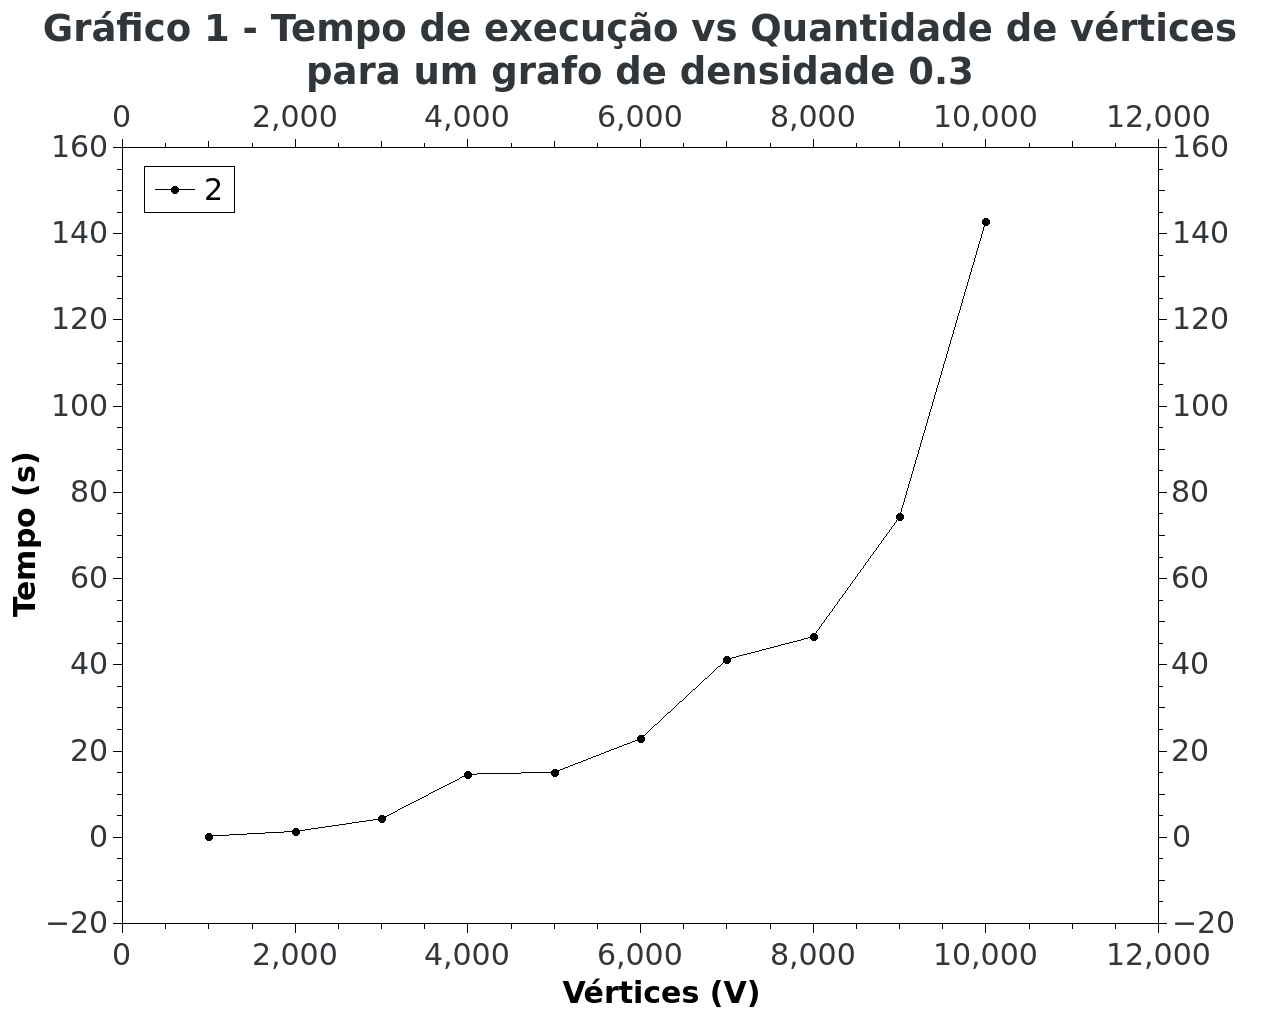
\includegraphics[scale=1.2]{graph1.png}
		\caption{Tempo de Execução em função da quantidade de vértices}
	\end{figure}
	
	\section{Análise de Resultado}
	
	Note que o crescimento da curva ocorre bem próximo do esperado, como a complexidade do algoritmo sugere, que é $O(|V|^2|E|)$. As pequenas variações ocorreram devido à característica única de cada grafo, que pode variar no padrão de adjcência dos vértices, assim como o grau de saída de cada vértice, entre outros fatores.
	
	\section{Conclusão}
	
	O objetivo do trabalho foi alcançado. O programa retorna para Gilmar a quantidade de ciclistas que podem sair das franquias e chegar nos cliente em segurança.
	
	O problema deste trabalho é um dos problemas clássicos da computação. O algoritmo escolhido, Dinic's, é robusto e eficiente. Entender como funciona todo o processo foi um trabalho arduoso, mas muito gratificante. Ademais, o trabalho foi divertido de ser feito e me fez aprender coisas além do problema de Fluxo Máximo, como por exemplo, utilizar a lista de adjacênias para armazenar as arestas e seus fluxos, e ainda sim conseguir acessar cada uma em $O(1)$ quando necessário.
	
	Uma melhora que pode ser feita neste programa é a manipulação de memória. Apesar de não possuir \textit{memory leak}, o programa aloca memória várias vezes, e isso torna a execução um pouco mais lenta, dado que a função \textit{malloc} tem um custo que não pode ser desconsiderao.
	
	\section{Referências}
	
	1. Maximum-flow problem
	
	Disponível em \url{https://en.wikipedia.org/wiki/Maximum_flow_problem}
	
	\hfill
	
	2. Flow network
	
	Disponível em \url{https://en.wikipedia.org/wiki/Flow_network}
	
	\hfill

	3. Dinic's Algorithm
	
	Disponível em \url{https://en.wikipedia.org/wiki/Dinic%27s_algorithm}
	
	\hfill
	
	4. Gerador de Grafos
	
	Disponível em \url{https://gist.github.com/bwbaugh/4602818#file-random_connected_graph-py}
	
	\hfill
	
	5. CSE 202: Design and Analysis of Algorithms
	
	Disponível em \url{https://cseweb.ucsd.edu/classes/sp11/cse202-a/lecture13-final.pdf}
	
	\hfill
	
	6. Level graph
	
	Disponível em \url{https://en.wikipedia.org/wiki/Level_structure}
	
	\hfill
	
	7. CS261: A Second Course in Algorithms
	
	Disponível em: \url{http://theory.stanford.edu/~tim/w16/l/l2.pdf}

\end{document}